\chapter{معالجة الأحداث (\textenglish{Event handling})}

معالجة الأحداث هو من أهم الأساسيات في الـ\textenglish{SDL}.\\
و ربّما قد يكون الشطر الأكثر شغفاً لاكتشافه. لأنه انطلاقا من هنا ستبدأ فعلاً في التحكّم في تطبيقك.

كلّ من مرفقات الحاسوب (فأرة، لوحة مفاتيح، \dots) قادرة على إنتاج حدث. سنتعلّم كيف نستقبل كل حدث و نتعامل معه. تطبيقك سيصبح أخيراً تفاعليّا !

فعلياً، ما هو الحدث ؟ الحدث هو عبارة عن إشارة
(\textenglish{signal})
يتم إرسالها عن طريق إحدى مرفقات الحاسوب 
(\textenglish{peripherals})
(أو عن طريق نظام التشغيل بذاته) إلى التطبيق. هذه أمثلة عن بعض الأحداث المألوفة :

\begin{itemize}
	\item حينما يضغط المُستعمل على زر من لوحة المفاتيح.
	\item و أيضاً حينما ينقر بالفأرة.
	\item حينما يحرّك الفأرة.
	\item حينما يقوم بتصغير النافذة.
	\item حينما يطلب إغلاق النافذة.
	\item إلى آخره.
\end{itemize}

الهدف من هذا الفصل هو تعلّم كيفية معالجة الأحداث. يمكنك أخيراً القول للحاسوب : "إذا نقر المستعمل في هذا المكان، قم بفعل كذا، و إن لم يفعل، قم بكذا. إذا حرّك الفأرة، قم بكذا. إذا ضغط على الزر
\InlineCode{Q}،
أوقف البرنامج. إلخ".

\section{مبدأ عمل الأحداث}

لنتعوّد على الأحداث، سنتعلّم كيف نتعامل مع أسهل حدث :
\textbf{طلب غلق البرنامج}.
هذا حدث يـُنتجُ حينما يقوم المستعمل بالنقر على الزر
\InlineCode{X} :

\begin{figure}[H]
	\centering
	
\includegraphics[width=0.05\textwidth]{Chapter_III-4_Close}
\end{figure}

إنه فعلاً الحدث الأكثر سهولة. إضافة على ذلك، هو حدث قد استعملته سابقاً دون أن تعلم بذلك لأنه متواجد في الدالة 
\InlineCode{pause} !\\
بالفعل، دور هذه الدالة هو انتظار المستعمل حتّى يقررّ غلق البرنامج، لأننا لو لم نستعملها كانت النافذة لتظهر و تختفي بسرعة البرق !

\begin{information}
يمكنك من الآن نسيان الدالة
\InlineCode{pause}.
قم بحذفها من الشفرة المصدرية لأننا سنتعلّم كيف نكتب محتواها بأنفسنا.
\end{information}

\subsection{متغيّر الحدث}

لمعالجة الأحداث، ستحتاج إلى التصريح عن متغيّر (واحد فقط، كن متأكدا) من نوع 
\InlineCode{SDL\_Event}.\\
فلتقم بتسميته بالاسم الذي يحلو لك، أنا سأسمّيه 
\InlineCode{event}،
و هي تعني "حدث" بالإنجليزيّة.

\begin{Csource}
SDL_Event event;
\end{Csource}

من أجل اختبارات الشفرة، سنستعمل دالة
\InlineCode{main}
بسيطة للغاية تقوم بإظهار نافذة فقط، مثلما رأينا في الفصول الأولى. هذا ما يجب أن تبدو عليه الدالة
\InlineCode{main} :

\begin{Csource}
int main(int argc, char *argv[])
{
	SDL_Surface *screen = NULL;
	SDL_Event event; // This variable will help us to manage the events
	SDL_Init(SDL_INIT_VIDEO);
	screen = SDL_SetVideoMode(640, 480, 32, SDL_HWSURFACE);
	SDL_WM_SetCaption("Gestion des événements en SDL", NULL);
	SDL_Quit();
	return EXIT_SUCCESS;
}
\end{Csource}

إذا، هي شفرة بدائية جداً، و هي لا تحوي سوى شيء جديد : تعريف المتغير
\InlineCode{event}
الذي سنستعين به قريباً.

جرّب الشفرة : مثلما توقّعنا، يجدر بالنافذة أن تظهر و تختفي في لحظة.

\subsection{حلقة الأحداث}

حينما نريد انتظار حدث، نستعمل غالباً حلقة. هذه الحلقة التكرارية تستمر في الاشتغال مادُمنا لم نستقبل الحدث المـُراد.\\
يجب علينا أن نستعمل متغيراً منطقياً لكي يحدد لنا ما إن كان علينا البقاء في الحلقة أو الخروج منها.\\
أنشئ هذا المتغير و سمّه مثلا
\InlineCode{cont}\footnote{
إذا كنت تفكّر في تسميته
\InlineCode{continue}
فلا تفعل، لأنّها كلمة مفتاحيّة (محجوزة)، و بالتالي لا يمكن استخدامها كاسم لمتغيّر.} :

\begin{Csource}
int cont = 1;
\end{Csource}

هذا المتغير المنطقي يأخذ القيمة 1 في البداية لأننا نريد للحلقة أن تتكرر مادام المتغير
\InlineCode{cont}
يحمل هذه القيمة (صحيح). ما إن يأخذ المتغير المنطقي القيمة 0 (خطأ)، نخرج من الحلقة و يتوقف البرنامج.

هذا ما تبدو عليه الحلقة :

\begin{Csource}
while (cont)
{
	// Dealing with the event
}
\end{Csource}

هكذا إذاً : لدينا لحدّ الآن حلقة غير منتهية لا تنتهي إلا إذا أخذ المتغير 
\InlineCode{cont}
القيمة 0. الأكثر أهمية هو ما نكتبه في داخل تلك الحلقة.

\subsection{استرجاع الحدث}

الآن سنقوم باستدعاء دالة من الـ\textenglish{SDL}
لكي نتحقق ما إن تم إنتاج حدث.\\
لدينا دالتان للقيام بهذا العمل، لكن كلا منهُما تعمل بطريقة مختلفة عن الأخرى :

\begin{itemize}
	\item \InlineCode{SDL\_WaitEvent} :
	تقوم بانتظار إنتاج حدث. هذه الدالة نقول عنها تعطيلية لأنها توقف عمل البرنامج مادام لم يتم إنتاج أي حدث.
	\item \InlineCode{SDL\_PollEvent} :
	هذه الدالة تقوم بنفس العمل لكنها ليست تعطيلية. لأنها تُخبرنا ما إن تم إنتاج حدث أم لا، فإن لم يكن هناك أي حدث فإنها تعيد التحكّم إلى البرنامج مباشرة.
\end{itemize}

هاتان الدالّتان مهمّتان، لكن في حالتين مختلفتين.\\
لتبسيط الأمور، إذا استعملت 
\InlineCode{SDL\_WaitEvent}
فإن برنامجك لن يـُتعب كثيراً المـُعالج لأنه سيتوقف مـُنتظراً إنتاج حدث.\\
بالمـُقابل، إذا استعملت 
\InlineCode{SDL\_PollEvent}،
سيقوم البرنامج بالعمل على الحلقة
\InlineCode{while}
و استدعاء الدالة 
\InlineCode{SDL\_PollEvent}
بشكل غير معرّف إلى حين إنتاج حدث مُعين. و بهذا تستعمل المُعالج  بنسبة 100
\%.

\begin{question}
لكن ألا يجب أن نستعمل دائماً الدالة 
\InlineCode{SDL\_WaitEvent}
بما أنها لا تستعمل المـُعالج كثيراً~؟
\end{question}

كلّا، لأنه توجد حالات لا يمكن الاستغناء فيها عن الدالة 
\InlineCode{SDL\_PollEvent}.
و هي حالة الألعاب التي يتم فيها تحديث الشاشة حتى و إن لم يكن هناك أي حدث.\\
فلنأخذ مثلاً اللعبة 
\textenglish{Tetris} :
تقوم الكتل بالنزول لوحدها، لا يحتاج المُستعمل إلى إنتاج حدث من أجل حصول هذا الأمر ! لو استعملنا
\InlineCode{SDL\_WaitEvent}،
سيبقى البرنامج مـُعطّلا و لن تتمكّن من تحديث الشاشة لإنزال الكتل !

\begin{question}
ماذا تفعل
\InlineCode{SDL\_WaitEvent}
لكي لا تستهلك من الـمُعالج كثيراً ؟\\
فبعد كل شيء، الدالة مُجبرة على البقاء في حلقة غير منتهية لكي تختبر كلّ الوقت ما إن كان هناك حدث أم لا، أليس كذلك ؟
\end{question}

الحقيقة أنني كنت أطرح هذا السؤال قبل وقت قليل. الإجابة معقّدة قليلاً لأنها تخصّ الطريقة التي يتحكّم فيها النظام بالعمليّات 
(\textenglish{Processes})
(البرامج التي هي في طور الاشتغال).\\
إذا كنت تريد -لكنّي سأتحدّث بسرعة-، بالنسبة للدالة 
\InlineCode{SDL\_WaitEvent}،
عمليّة البرنامج تُوضع في طور الانتظار.\\
إذا فإن البرنامج لا يعمل عليه المعالج بعد تلك اللحظة.\\
سيتم "إيقاظه" من طرف نظام التشغيل حينما يتم إنتاج حدث. يعني أن المعالج سيعود إلى العمل على البرنامج في هذه اللحظة. هذا ما يشرح لِمَا لا يستهلك البرنامج من المعالج شيئا بينما يكون في طور انتظار الحدث.

أدري أن هذه المفاهيم تبدو مجرّدة لك الآن. لكنك لست مُجبراً على فهم كل هذا الآن لأنك ستبدأ في التأقلم مع هذه المعلومات شيئاً في شيئاً مع التطبيق.\\
الآن سنستعمل 
\InlineCode{SDL\_WaitEvent}
لأن البرنامج سيبقى بسيطا باستخدامها. على أي حال فالتعامل مع هاتين الدالتين لن يتغير من واحدة إلى أخرى.

يجب أن تبعث للدالة عنوان المتغير 
\InlineCode{event}
الذي يقوم بتخزين الحدث.\\
بما أن هذا المتغير ليس عبارة عن مؤشّر (أعد رؤية طريقة التصريح به أعلاه)، سنستعمل الاشارة
\InlineCode{\&}
قبل اسم المتغير و ذلك لنُعطي عنوانه :

\begin{Csource}
SDL_WaitEvent(&event);
\end{Csource}

بعد استدعاء هذه الدالة، المتغير
\InlineCode{event}
يحتوي إجبارياً حدثاً ما.

\begin{information}
هذه الحالة ليست نفسها لو استعملنا
\InlineCode{SDL\_PollEvent}
لأن هذه الأخيرة قادرة على أن تُرجع لنا : "لا يوجد أي حدث".
\end{information}

\subsection{تحليل الحدث}

الآن نحن نتوفر على متغير
\InlineCode{event}
يحتوي على معلومات حول الحدث الذي تم إنتاجه.\\
يجب أن نرى المركّب
\InlineCode{event.type}
و نختبر قيمته. غالبا ما نستعمل
\InlineCode{switch}
لاختبار الحدث.

\begin{question}
لكن كيف لنا أن نعرف ما هي القيمة الموافقة للحدث "أغلق البرنامج" مثلا ؟
\end{question}

الـ\textenglish{SDL}
توفّر لنا بعض الثوابت، مما يسهّل كثيراً كتابة البرنامج. هذه الثوابت كثيرة العدد (بقدر وجود أحداث ممكن حصولها في الحاسوب). سنتعرّف على هذه الثوابت بتقدّمنا في هذا الفصل.

\begin{Csource}
while (cont)
{
	SDL_WaitEvent(&event); // Getting the event in "event"
	switch(event.type) // Testing the event's type
	{
		case SDL_QUIT: // If it's a quit event
		cont = 0;
		break;
	}
}
\end{Csource}

هكذا تعمل الشفرة :

\begin{enumerate}
	\item ما إن يتم انتاج حدث، تُرجع الدالة 
	\InlineCode{SDL\_WaitEvent}
	الحدث في المتغير 
	\InlineCode{event}.
	\item نقوم بتحليل نوع الحدث بالاستعانة بـ\InlineCode{switch}.
	نوع الحدث موجود في
	\InlineCode{event.type}.
	\item نختبر بمساعدة 
	\InlineCode{case}
	نوع الحدث. لحدّ الآن، نحن لا نتحقق إلا إذا ما كان الحدث يوافق
	\InlineCode{SDL\_QUIT}
	(طلب إغلاق البرنامج)، لأنّها الحالة الوحيدة التي تهمّنا.
	\item إذا كان الحدث هو 
	\InlineCode{SDL\_QUIT}،
	فهذا يعني أن المستعمل طلب إغلاق البرنامج. في هذه الحالة، نعطي للمتغير المنطقي
	\InlineCode{cont}
	القيمة 0. في الدورة القادمة للحلقة، سيكون الشرط غير محقق، فيتوقف تشغيل البرنامج.
	\item إذا لم يكن الحدث هو 
	\InlineCode{SDL\_QUIT}،
	مما يعني أنه قد حدث شيء آخر : قام المستعمل بالضغط على زر، بالنقر على الفأرة أو ببساطة قام بتحريك الفأرة داخل النافذة. و بما أن هذه الأحداث لا تهمّنا، لن نقوم بمعالجتها. لن نقوم إذا بأي شيء : تقوم الحلقة بالانتقال في كلّ مرة إلى دورة جديدة ننتظر فيها وقوع حدث جديد (بمعنى آخر، نعود إلى النقطة 1).
\end{enumerate}

ما أنا أشرحه لك الآن هو أمر مهم جداً. إذا فهمت هذه الشفرة، فقد فهمت كلّ شيء و سيكون باقي الفصل سهلاً للغاية.

\subsection{الشفرة الكاملة}

\begin{Csource}
int main(int argc, char *argv[])
{
	SDL_Surface *screen = NULL;
	SDL_Event event; // The event's variable
	int cont = 1; // A boolean for the loop
	SDL_Init(SDL_INIT_VIDEO);
	screen = SDL_SetVideoMode(640, 480, 32, SDL_HWSURFACE);
	SDL_WM_SetCaption("Gestion des événements en SDL", NULL);
	while (cont) // While the variable's value is 
	{            // not equal to 0
		SDL_WaitEvent(&event); // We wait for an event that we recuperate in "event"
		switch(event.type) // Testing the event's type
		{
			case SDL_QUIT: // If it's a quit event
			cont = 0; // We change the boolean value so we go out from the loop.
			break;
		}
	}
	SDL_Quit();
	return EXIT_SUCCESS;
}
\end{Csource}

هاهي الشفرة الكاملة. لا يوجد شيء صعب : إذا قمت بمتابعة الفصل إلى الآن، يجدر بك أن تكون قد فهمت كلّ شيء. على أي حال فقد لاحظت أنّنا لم نقم إلا بإعادة كتابة ما تقوم به الدالة 
\InlineCode{pause}.
قارن هذه الشفرة بما تقوم به الدالة
\InlineCode{pause} :
هو نفس الشيء، إلا أنه في هذه الحالة نقوم بوضع كلّ شيء في الدالة
\InlineCode{main}.
بالطبع، من المستحسن نقل الشفرة إلى دالة أخرى على حدى كـ\InlineCode{pause}،
لأن ذلك سيقلّل من حجم الدالة
\InlineCode{main}
و يجعلها أفضل من ناحية فهم الشفرة.

\section{لوحة المفاتيح}

سنقوم الآن بدراسة الأحداث التي تـُنتج عن طريق لوحة المفاتيح.

إذا فهمت بداية الفصل، فلن تواجه أي مشكل في التعامل مع أي نوع من الأحداث. لا يوجد ماهو أسهل.

لماذا هذا سهل ؟ لأننا الآن فهمنا طريقة عمل الحلقة التكرارية غير المنتهية، كل ما ستقوم بفعله هو إضافة بعض الحالات إلى الـ\InlineCode{switch}
من أجل تحليل أنواع أخرى من الأحداث. لا يفترض أن يكون هذا الأمر صعباً.

\subsection{أحداث لوحة المفاتيح}

يوجد نوعان من الأحداث التي يمكن توليدها عن طريق لوحة المفاتيح :

\begin{itemize}
	\item \InlineCode{SDL\_KEYDOWN} :
حينما يتم بدأ الضغط على زر من لوحة المفاتيح.
	\item \InlineCode{SDL\_KEYUP} :
حينما يتحرر زر لوحة المفاتيح.
\end{itemize}

لماذا يوجد حدثان إثنان ؟\\
لأننا حينما نضغط على زر، يحدث أمران : شدّ الزر إلى الأسفل
(\InlineCode{SDL\_KEYDOWN})
ثمّ تحريره 
(\InlineCode{SDL\_KEYUP}).
تسمح لنا الـ\textenglish{SDL}
بتحليل كل من هذين الحدثين على حدى، و هذا أمر عملي جداً، سترى ذلك.

لحدّ الآن سنكتفي بتحليل الحدث
\InlineCode{SDL\_KEYDOWN}
(الضغط على الزر) :

\begin{Csource}
while (cont)
{
	SDL_WaitEvent(&event);
	switch(event.type)
	{
		case SDL_QUIT:
		cont = 0;
		break;
		case SDL_KEYDOWN: // If we press a button
		cont = 0;
		break;
	}
}
\end{Csource}

إذا ضغطنا على أي زر سيتوقف البرنامج، جرّب ذلك !

\subsection{استرجاع رمز الزر}

معرفة أنه تم الضغط على زر من لوحة المفاتيح هو أمر جيد، لكن معرفة أي الأزرار تم الضغط عليه بالضبط هو أمر أحسن !

يمكننا معرفة الزر الذي تم الضغط عليه بفضل مركّب مركّب مركّب المتغيّر (أوف !) و الذي يُدعى 
\InlineCode{event.key.keysym.sym}.
 هذا المتغير يحتوي قيمة الزر الذي تم الضغط عليه (و هو يعمل حتى في الحين الذي نحرر فيه الزر
\InlineCode{SDL\_KEYUP}).

\begin{information}
الشيء الجيد هو أن الـ\textenglish{SDL}
تسمح باسترجاع هذه القيمة من كل أزرار لوحة المفاتيح و التي تتضمّن على الحروف و الأرقام، و كذلك الأزرار 
\InlineCode{Esc}، \InlineCode{Print scr.}، \InlineCode{Del}، \InlineCode{Enter}، \dots
إلخ.
\end{information}

يوجد ثابت من أجل كل زر في اللوحة. يمكنك الاطلاع على قائمة هذه الثوابت من خلال الملفات التوثيقيّة الخاصة بالـ\textenglish{SDL}،
الّتي من المفترض أنّك قد نزلتها مع المكتبة 
\textenglish{SDL}.\\
إن لم تفعل، فأنصحك بالتوجه إلى موقع المكتبة و تحميل هذه الملفات لأنها مهمّة للغاية.

ستجد قائمة أزرار لوحة المفاتيح في القسم
"\textenglish{Keysym definitions}".
هذه القائمة طويلة جداً و لا يمكنني تقديمها هنا و لهذا عليك تصفح التوثيق من الموقع مباشرة.

\url{http://www.siteduzero.com/uploads/fr/ftp/mateo21/sdlkeysym.html}

هذه الملفات مُحررة باللغة الانجليزية، و هي غير متوفرة بلغة أخرى. إذا كنت تريد البرمجة حقّا، فمن الواجب أن تجيد هذه اللغة لأنّ  كلّ الملفات التوثيقيّة مكتوبة بها، فلا يمكنك أبدا تجاوزها !

يوجد في اللائحة جدولان : واحد كبير (في البداية) و آخر صغير (في النهاية). نحن الآن نهتم بالجدول الأكبر.\\
في العمود الأول تجد الثابت، في العمود الثاني تجد القيمة الموافقة له بالـ\textenglish{ASCII}
و أخيرا في العمود الثالث تجد وصفاً للزر.\\
لاحظ أن بعض الأزرار كـ\InlineCode{Maj}
(\InlineCode{Shift})
لا تملك قيمة
\textenglish{ASCII}
موافقة لها.

فلنأخذ مثلاً الزر
\InlineCode{Esc}.
يمكننا معرفة ما إن كان هذا الزر مضغوطاً كالتالي :

\begin{Csource}
switch (event.key.keysym.sym)
{
	case SDLK_ESCAPE: // Pressing Escape button lets us quit the program
	cont = 0;
	break;
}
\end{Csource}

\begin{information}
أستعمل
\InlineCode{switch}
من أجل الاختبار الأول لكن كان بإمكاني استعمال
\InlineCode{if}
ببساطة.\\
في كلّ مرة أميل إلى الاستعانة بالـ\InlineCode{switch}
حينما أعالج الأحداث لأنني أختبر الكثير من القيم المختلفة (عملياً، يتوفر لدينا الكثير من الحالات في الـ\InlineCode{switch}،
على عكس هذا المثال).
\end{information}

هذه حلقة حدث كاملة يمكنك تجريبها :

\begin{Csource}
while (cont)
{
	SDL_WaitEvent(&event);
	switch(event.type)
	{
		case SDL_QUIT:
		cont = 0;
		break;
		case SDL_KEYDOWN:
		switch (event.key.keysym.sym)
		{
			case SDLK_ESCAPE: 
			cont = 0;
			break;
		}
		break;
	}
}
\end{Csource}

\begin{information}
هذه المرة، يتوقف البرنامج حينما نضغط على الزر
\InlineCode{Esc}
أو إذا نقرنا على الرمز
\InlineCode{X}
أعلى النافذة. و الآن بما أنك تعرف كيف تغلق البرنامج بالضغط على زر معين، أنت مـُخوّل لاستعمال وضع الشاشة الكاملة إذا كان هذا ممتعا لك (استعمل العـَلم
\InlineCode{SDL\_FULLSCREEN}
في الـ\InlineCode{SDL\_SetVideoMode}،
كتذكير).\\
سابقاً كنت قد منعتك من استعمال هذا الأسلوب في العرض خشية أننا لن نتمكن من غلق البرنامج (لأنه لن يظهر لنا زرّ الإغلاق الّذي نضغط عليه لإيقاف البرنامج !)
\end{information}

\section{تمرين : تحريك \textenglish{Zozor} بواسطة لوحة المفاتيح}

أنت الآن قادر على تحريك صورة في النافذة بواسطة لوحة المفاتيح !\\
هذا تمرين مهمّ جداً سيسمح لنا بالتعرف على كيفية استعمال الـ\textenglish{double buffering}
و الاستعمال المتكرر للأزرار.\\
إضافة إلى ذلك، ما أنا بصدد تعليمه لك هو قاعدة كل ألعاب الفيديو التي تُصنع بالـ\textenglish{SDL}.
و لهذا فإن
\textbf{هذا التمرين ليس اختياريا}
! أدعوك لقراءته و محاولة حلّه بشكل جدّي.

\subsection{تحميل الصورة}

في البداية، سنقوم بتحميل صورة. سيكون الأمر بسيطاً : سنعيد استعمال صورة 
\textenglish{Zozor}
المُستعملة في الفصل السابق.\\
أنشئ المساحة
\InlineCode{zozor}،
حمّل الصورة و حوّل خلفيتها إلى اللون الشفاف (أذكرك بأن صيغة الصورة هي 
\textenglish{BMP}).

\begin{Csource}
zozor = SDL_LoadBMP("zozor.bmp");
SDL_SetColorKey(zozor, SDL_SRCCOLORKEY, SDL_MapRGB(zozor->format, 0, 0, 255));
\end{Csource}

بعد ذلك، الشيء الأكثر أهمية، يجب عليك إنشاء متغير من نوع
\InlineCode{SDL\_Rect}
لتقوم بحِفظ مركبات
\textenglish{Zozor}.

\begin{Csource}
SDL_Rect positionZozor;
\end{Csource}

أنصحك بإعطاء قيم ابتدائية للمركبات، ضع مثلا
\InlineCode{x = 0}
و 
\InlineCode{y = 0}
(الوضعية أعلى يسار النافذة) أو قم بـِمـَرْكَـزَة
\textenglish{Zozor}
في وسط النافذة كما قمت بتعليمك هذا من قبل.

\begin{Csource}
// We center Zozor in the screen
zozorPosition.x = screen->w / 2 - zozor->w / 2;
zozorPosition.y = screen->h / 2 - zozor->h / 2;
\end{Csource}

\begin{critical}
يجب عليك تهيئة المتغير 
\InlineCode{zozorPosition}
\textit{بعد}
تحميل المساحتين 
\InlineCode{screen}
و 
\InlineCode{zozor}.
في الواقع، سأستعمل العرض 
\InlineCode{w}
و الارتفاع 
\InlineCode{h}
لهاتين المساحتين من أجل حساب الموقع المركزي لـ\textenglish{Zozor}
في الشاشة، و لهذا كان لازما أن يتم تهيئة هاتين المساحتين من قبل.
\end{critical}

إذا كنت قد تدبّرت أمرك جيّدا، يجدر أن يظهر 
\textenglish{Zozor}
في وسط النافذة.

\begin{figure}[H]
	\centering
	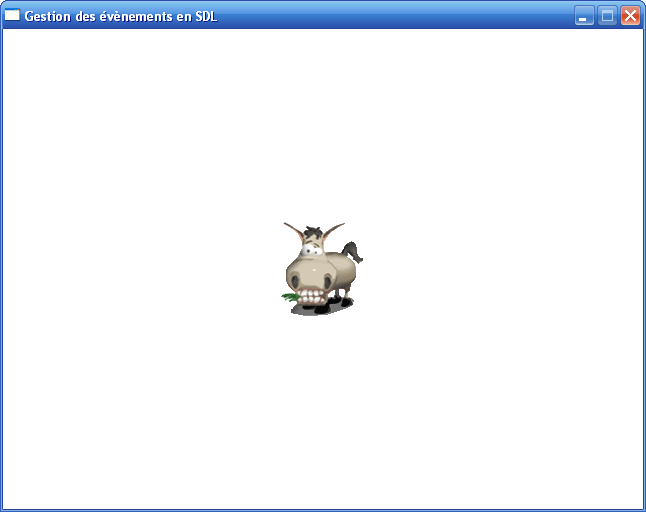
\includegraphics[width=0.6\textwidth]{Chapter_III-4_Window-Zozor}
\end{figure}

لقد اخترت هذه المرة وضع خلفية بيضاء (قمت بـ\InlineCode{SDL\_FillRect})
لكن هذا ليس واجباً.

\subsection{مخطط البرمجة بالأحداث}

حينما تقوم ببرمجة برنامج يتفاعل مع الأحداث (كما سنقوم بفعله الآن)، يجب عليك اتّباع نفس "المخطط" في غالب الأحيان.\\
يجدر بك 
\textit{حفظ هذا المخطط عن ظهر قلب} :

\begin{Csource}
while (cont)
{
	SDL_WaitEvent(&event);
	switch(event.type)
	{
		// Managing the events of type SOMETHING
		case SDL_SOMETHING:
		// Managing the events of type ANOTHERTHING
		case SDL_ANOTHERTHING:
	}
	// We clear the screen
	SDL_FillRect(screen, NULL, SDL_MapRGB(screen->format, 255, 255, 255)); 
	// We do all the necessary SDL_BlitSurface to past the surfaces on the screen
	// We update the display
	SDL_Flip(screen);
}
\end{Csource}

سأقدّم لك أهمّ السطور التي تكوّن الحلقة الرئيسية في برنامج 
\textenglish{SDL}.\\
سنستمر في تشغيل الحلقة مادام لم يتم طلب غلق البرنامج.

\begin{enumerate}
	\item ننتظر حدثاً
	(\InlineCode{SDL\_WaitEvent})
	أو نقوم بالتحقق من وجود حدث لكن لا نقوم بانتظار حدوث واحد 
	(\InlineCode{SDL\_PollEvent}).
	حاليا نكتفي باستعمال 
	\InlineCode{SDL\_WaitEvent}.
	\item نستعمل 
	\InlineCode{switch}
	(كبير) من أجل معرفة نوع الحدث الذي نحن نتعامل معه. نقوم بتحليل الحدث الّذي تلقّيناه ثم نقوم ببعض الحسابات و العمليات.
	\item ما إن نخرج من الـ\InlineCode{switch}،
	نحضّر عرضا جديدا لنقوم بإظهاره.
	\item أول شيء نفعله : نمسح الشاشة باستعمال
	\InlineCode{SDL\_FillRect}.
	إن لم نقم بذلك، ستبقى بعض "آثار" الشاشة السابقة في الشاشة الحالية مما يشوش المظهر.
	\item نقوم بعد ذلك بلصق كل المساحات على الشاشة.
	\item أخيرا، ما إن ننتهي من كل ذلك، نقوم بتحديث العرض من أجل المستعمل و ذلك باستدعاء الدالة
	\InlineCode{SDL\_Flip}.
\end{enumerate}

\subsection{معالجة الحدث \texttt{SDL\_KEYDOWN}}

لنرى الآن كيف نعالج الحدث 
\InlineCode{SDL\_KEYDOWN}.\\
هدفنا هو تحريك 
\textenglish{Zozor}
بواسطة لوحة المفاتيح باستعمال الأسهم التوجيهية. و لهذا سنقوم بتغيير مركباته في الشاشة بدلالة السهم الذي يضغط عليه المستعمل :

\begin{Csource}
switch(event.type)
{
	case SDL_QUIT:
	cont = 0;
	break;
	case SDL_KEYDOWN:
	switch(event.key.keysym.sym)
	{
		case SDLK_UP: // Up arrow
		zozorPosition.y--;
		break;
		case SDLK_DOWN: // Down arrow
		zozorPosition.y++;
		break;
		case SDLK_RIGHT: // Right arrow
		zozorPosition.x++;
		break;
		case SDLK_LEFT: // Left arrow
		zozorPosition.x--;
		break;
	}
	break;
}
\end{Csource}

أين وجدت أسماء الثوابت ؟  لقد وجدتها في التوثيق !\\
لقد اعطيتك قبل قليل الرابط الخاص بالتوثيق الّذي يعطي لائحة كل الأزرارفي لوحة المفاتيح : هنا وجدت ضالّتي. 

ما فعلناه هنا هو أمر بسيط جداً :

\begin{itemize}
	\item إذا ضغطنا على السهم "أعلى"، نقوم بإنقاص الترتيبة 
	(\InlineCode{y})
	الخاصة بـ\textenglish{Zozor}
	ببيكسل واحد من أجل جعله يصعد. لاحظ أننا لسنا مُجبرين على تحريكه ببيكسل واحد، يمكننا تحريكه بـ10 بيكسل في كلّ مرة.
	\item إذا توجهنا إلى الأسفل، سنقوم بزيادة الترتيبة
	(\InlineCode{y})
	لـ\textenglish{Zozor}.
	\item إذا توجهنا لليمين نزيد قيمة الفاصلة 
	(\InlineCode{x}).
	\item إذا توجهنا لليسار نقوم بإنقاص الفاصلة  
	(\InlineCode{x}).
\end{itemize}

و الآن ؟\\
بما أنني أعطيتك التوجيهات و حتى المخطط، يجدر بك أن تكون قادراً على كتابة الشفرة التي تسمح بتحريك
\textenglish{Zozor}
في النافذة !

\begin{Csource}
int main(int argc, char *argv[])
{
	SDL_Surface *screen = NULL, *zozor = NULL;
	SDL_Rect zozorPosition;
	SDL_Event event;
	int cont = 1;
	SDL_Init(SDL_INIT_VIDEO);
	screen = SDL_SetVideoMode(640, 480, 32, SDL_HWSURFACE);
	SDL_WM_SetCaption("Gestion des événements en SDL", NULL);
	// Loading Zozor
	zozor = SDL_LoadBMP("zozor.bmp");
	SDL_SetColorKey(zozor, SDL_SRCCOLORKEY, SDL_MapRGB(zozor->format, 0, 0, 255));
	zozorPosition.x = screen->w / 2 - zozor->w / 2;
	zozorPosition.y = screen->h / 2 - zozor->h / 2;
	while (cont)
	{
		SDL_WaitEvent(&event);
		switch(event.type)
		{
			case SDL_QUIT:
			cont = 0;
			break;
			case SDL_KEYDOWN:
			switch(event.key.keysym.sym)
			{
				case SDLK_UP: // Up arrow
				zozorPosition.y--;
				break;
				case SDLK_DOWN: // down arrow
				zozorPosition.y++;
				break;
				case SDLK_RIGHT: // Right arrow
				zozorPosition.x++;
				break;
				case SDLK_LEFT: // Left arrow
				zozorPosition.x--;
				break;
			}
			break;
		}
		// Clear the screen
		SDL_FillRect(screen, NULL, SDL_MapRGB(screen->format, 255, 255, 255));
		// We put zozor in its new position
		SDL_BlitSurface(zozor, NULL, screen, &zozorPosition);
		// Update the display
		SDL_Flip(screen);
	}
	SDL_FreeSurface(zozor);
	SDL_Quit();
	return EXIT_SUCCESS;
}
\end{Csource}

إنه من الضروري جداً الفهم الجيد لكيفية عمل الحلقة الرئيسية في البرنامج. يجب أن تكون قادراً على كتابتها بنفسك. استعن بالمخطط الذي أعطيتك إياه أعلاه إذا اقتضت الحاجة.

باختصار إذا، توجد حلقة كبيرة تُسمى "الحلقة الرئيسية في البرنامج". و هي لا تتوقف إلا إذا أعطينا للمتغير 
\InlineCode{cont}
القيمة 0.\\
في هذه الحلقة، نقوم أولا باسترجاع حدث لنقوم بمعالجته. نستعمل 
\InlineCode{switch}
من أجل تحديد نوع الحدث. بدلالة الحدث، نقوم بعمليات مختلفة. في حالتنا هذه، نقوم بتحديث مركبات وضعية
\textenglish{Zozor}
من أجل إعطاء انطباع أننا نقوم بتحريكه.

ثم بعد الـ\InlineCode{switch}
يجب عليك تحديث الشاشة كالتالي :

\begin{enumerate}
	\item أولاً، نمسح الشاشة باستعمال
	\InlineCode{SDL\_FillRect}
	(باستعمال لون خلفية يناسبك).
	\item ثم تقوم بتسوية المساحات على الشاشة. هنا، لم أحتج إلى لصق إلا
	\textenglish{Zozor}
	لأننا لا نحتاجه إلا هو كما هو واضح، و من المهم جداً أن نضع
	\textenglish{Zozor}
	في الموضع
	\InlineCode{zozorPosition} !
	لان هذا ما يصنع الفارق~: إذا كنتُ قد حدّثتُ
	\InlineCode{zozorPosition}
	كان
	\textenglish{Zozor}
	ليظهر في مكان آخر و بهذا نعتقد أننا غيّرنا مكانه كليا !
	\item أخيراً، و آخر شيء للقيام به :
	\InlineCode{SDL\_Flip}
	لكي نحدّث الشاشة من أجل المستعمل.
\end{enumerate}

و بهذا نتمكن من تحريك الحيوان إلى أي مكان نريده !

\begin{figure}[H]
	\centering
	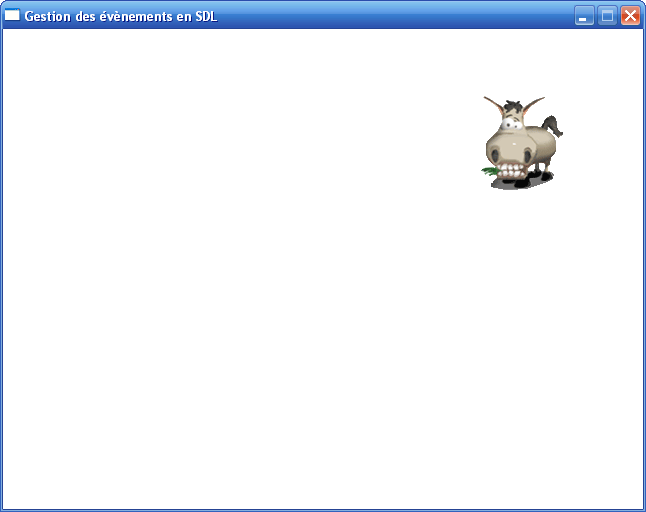
\includegraphics[width=0.6\textwidth]{Chapter_III-4_Window-Zozor-moved}
\end{figure}

\subsection{بعض التحسينات}

\subsubsection{تكرار الضغط على الأزرار}

لحد الآن، البرنامج يعمل لكنّه يُلزم تحرّك اللاعب أن يكون بيكسلا في المرّة الواحدة. نحن مُجبَرون على الضغط من جديد على الأسهم إذا أردنا التحرك مرة أخرى ببيكسل. لا أدري بالنسبة لك، لكنني أستمتع أحيانا بالبقاء ضاغطا على نفس الزر وقتا أطول لكي أحرك اللاعب بـ200 بيكسل.

على كل حال، من حسن الحظّ أن الدالة 
\InlineCode{SDL\_EnableKeyRepeat}
موجودة !\\
هذه الدالة تسمح بتفعيل الضغط المتكرر على الأزرار. فهي تحرّض الـ\textenglish{SDL}
على إعادة إنتاج حدث من نوع
\InlineCode{SDL\_KEYDOWN}
إذا بقي المستعمل ضاغطاً على نفس الزر لمدة من الزمن.

يمكنك استدعاء هذه الدالة أينما أردت، لكنني أنصحك باستدعائها قبل الحلقة الرئيسية للبرنامج. يمكن للدالة أخذ معاملين :

\begin{itemize}
	\item المدة (بالميلّي ثانية) التي يجدر بالزر أن يبقى فيها مضغوطاً قبل تفعيل تكرار الضغط على الأزرار.
	\item الأجل (بالميلّي ثانية) بين كل إنتاج لحدث
	\InlineCode{SDL\_KEYDOWN}
	و آخر ما إن يتم تفعيل تكرار الضغط على الأزرار.
\end{itemize}

المعامل الأول يشير إلى مدة الزمن التي يجدر بنا بعدها إنتاج تكرار الضغط على الأزرار في المرة الأولى. أما الثاني فيشير إلى الوقت اللازم ليتم إعادة إنتاج الحدث.\\
شخصياً، و من أجل أسباب ليونة التحرك، أعطي غالباً نفس القيمة للمعاملين. جرّب القيمة 10 ميلّي ثانية :

\begin{Csource}
SDL_EnableKeyRepeat(10, 10);
\end{Csource}

الآن، يمكنك البقاء ضاغطاً على نفس السهم. سترى أنّ هذا أحسن !

\subsubsection{العمل بالـ\textenglish{double buffering}}

انطلاقا من الآن، سيكون من الجيد تفعيل تقنية الـ\textenglish{double buffering}
الخاصة بالـ\textenglish{SDL}.
الـ\textenglish{double buffering}
هي تقنية مستعملة بكثرة في الألعاب. تسمح هذه التقنيّة بتجنب التقطع في الصورة.\\
لِـمَا تتقطع الصورة ؟ لأنه حينما نرسم في الشاشة، المستعمل "يرى" كيف ترسم و بهذا يرى كيف تُمسح الشاشة. حتى وإن جرت العملية بسرعة فإن مخّ الإنسان يلتقط إشارات خفيفة و قد تكون مزعجة.

تقنية الـ\textenglish{double buffering}
تعمل على استخدام "شاشتين" : واحدة حقيقية (التي يراها المستعمل في شاشة الحاسوب) و أخرى افتراضية (هي صورة يقوم الحاسوب بإنشائها في الذاكرة).

هاتان الشاشتان تتناوبان : الشاشة
\textenglish{A}
تظهر في حين تحضّر الشاشة
\textenglish{B}
الصورة القادمة في  الخلفية. لاحظ الصورة التالية :

\begin{figure}[H]
	\centering
	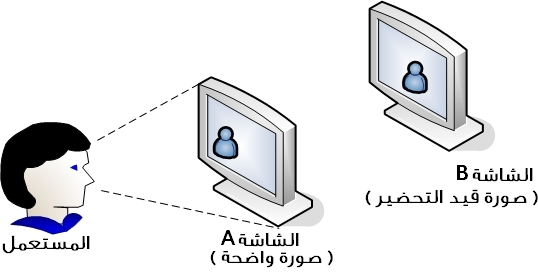
\includegraphics[width=0.5\textwidth]{Chapter_III-4_Double-buffering-1}
\end{figure}

ما إن يتم رسم الصورة في الشاشة الخلفية (الشاشة 
\textenglish{B})،
نقوم بقلب الشاشتين و ذلك باستدعاء الدالة
\InlineCode{SDL\_Flip}.

\begin{figure}[H]
	\centering
	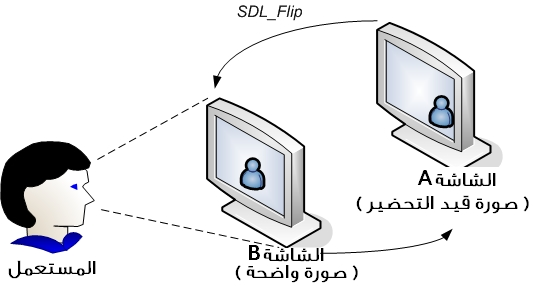
\includegraphics[width=0.5\textwidth]{Chapter_III-4_Double-buffering-2}
\end{figure}

الشاشة
\textenglish{A}
تصبح شاشة خلفية و تقوم بتحضير الصورة القادمة، بينما يتم إظهار الصورة في الشاشة
\textenglish{B}
و يراها المستعمل. النتيجة : لا يوجد تقطع في الصورة !

لتحقيق هذا كل ما عليك فعله هو تحميل وضع العرض بإضافة العَلم 
\InlineCode{SDL\_DOUBLEBUF} :

\begin{Csource}
screen = SDL_SetVideoMode(640, 480, 32, SDL_HWSURFACE | SDL_DOUBLEBUF);
\end{Csource}

لا يوجد شيء آخر لتغييره في الشفرة المصدرية.

\begin{information}
 الـ\textenglish{double buffering}
هي تقنية معروفة جداً في البطاقة الرسومية
(\textenglish{Graphics card})
 للحاسوب. ما أقصده هو أن الجهاز هو من يتحكم في كلّ شيء، و يتم ذلك بسرعة جدّ فائقة.
\end{information}

ستتساءل ربّما لماذا كنا قد استعملنا
\InlineCode{SDL\_Flip}
من قبل دون الـ\textenglish{double buffering} ؟\\
الواقع أن لهذه الدالة وظيفتين :

\begin{itemize}
	\item إذا كانت الـ\textenglish{double buffering}
	مفعّلة، فستتحكم في تناوب الشاشتين.
	\item أما إن كانت غير مفعّلة، فهي تتحكم في تحديث النافذة يدويا. هذه التقنية تعمل في حالة كان البرنامج لا يقدّم حركية كبيرة، و لكن في غالبية الألعاب، أنصحك بتفعيلها.
\end{itemize}

من الآن و صاعداً، سأقوم بتفعيل هذه التقنية في كل الشفرات المصدرية التي أكتبها (لأنها لا تكلف الكثير و تقدم الكثير، فمما نشكي ؟)

إليك الشفرة المصدرية الكاملة التي تسمح باستعمال الـ\textenglish{double buffering}
و تكرار الضغط على الأزرار. إنها مشابهة للشفرة التي رأيناها قبل قليل، لقد قمت فقط بإضافة بعض التعليمات التي نحن بصدد تعلّمها :

\begin{Csource}
int main(int argc, char *argv[])
{
	SDL_Surface *screen = NULL, *zozor = NULL;
	SDL_Rect zozorPosition;
	SDL_Event event;
	int cont = 1;
	SDL_Init(SDL_INIT_VIDEO);
	zozorPosition = SDL_SetVideoMode(640, 480, 32, SDL_HWSURFACE | SDL_DOUBLEBUF); // Double buffering
	SDL_WM_SetCaption("Gestion des événements en SDL", NULL);
	zozor = SDL_LoadBMP("zozor.bmp");
	SDL_SetColorKey(zozor, SDL_SRCCOLORKEY, SDL_MapRGB(zozor->format, 0, 0, 255));
	zozorPosition.x = screen->w / 2 - zozor->w / 2;
	zozorPosition.y = screen->h / 2 - zozor->h / 2;
	SDL_EnableKeyRepeat(10, 10); // Enabling keys repetition
	while (cont)
	{
		SDL_WaitEvent(&event);
		switch(event.type)
		{
			case SDL_QUIT:
			cont = 0;
			break;
			case SDL_KEYDOWN:
			switch(event.key.keysym.sym)
			{
				case SDLK_UP:
				zozorPosition.y--;
				break;
				case SDLK_DOWN:
				zozorPosition.y++;
				break;
				case SDLK_RIGHT:
				zozorPosition.x++;
				break;
				case SDLK_LEFT:
				zozorPosition.x--;
				break;
			}
			break;
		}
		SDL_FillRect(screen, NULL, SDL_MapRGB(screen->format, 255, 255, 255));
		SDL_BlitSurface(zozor, NULL, screen, &zozorPosition);
		SDL_Flip(screen);
	}
	SDL_FreeSurface(zozor);
	SDL_Quit();
	return EXIT_SUCCESS;
}
\end{Csource}

\section{الفأرة}

ربما تعتقد أن التحكّم في الفأرة أمر أكثر تعقيداً من التحكم في لوحة المفاتيح ؟\\
كلا، بل حتّى أن الأمر أسهل، سترى !

سترى بأن الفأرة يمكن لها أن تُنتج ثلاثة أنواع مختلفة من الأحداث.

\begin{itemize}
	\item \InlineCode{SDL\_MOUSEBUTTONDOWN}
	حينما ننقر بالفأرة، و هذا الحدث يوافق اللحظة الذي يكون فيه زر الفأرة مضغوطاً.
	\item \InlineCode{SDL\_MOUSEBUTTONUP} :
	حينما نحرر زر الفأرة. كل هذا يعمل وفقاً لنفس المبدأ التي تعمل به أزرار لوحة المفاتيح : يوجد ضغط للزر ثم تحرير لهذا الأخير.
	\item \InlineCode{SDL\_MOUSEMOTION} :
	حينما نقوم بتحريك الفأرة. في كل مرة تقوم فيها الفأرة بالتحرك في النافذة (هذا لا يتم إلا بيكسلا ببيكسل)، يتم إنتاج الحدث 
	\InlineCode{SDL\_MOUSEMOTION} !
\end{itemize}
 
سنبدأ أولا بالعمل على النقر على الفأرة و بشكل خاص على
\InlineCode{SDL\_MOUSEBUTTONUP}.
لن نعمل مع\\
الـ\InlineCode{SDL\_MOUSEBUTTONDOWN}،
لكنك تعرف بأن الطريقة لا تختلف إلا أن الحدث الأخير يُنتج قبل الحدث الآخر.\\
سنعلم لاحقاً كيف نتعامل مع الحدث
\InlineCode{SDL\_MOUSEMOTION}.

\subsection{معالجة نقرات الفأرة}

سنقوم إذا باستقبال حدث من نوع
\InlineCode{SDL\_MOUSEBUTTONUP}
(النقر بالفأرة) ثم نرى ما يمكننا استرجاعه من معلومات.\\
كالعادة، يجدر بنا إضافة حالة
\InlineCode{case}
في الـ\InlineCode{switch}
كالتالي :

\begin{Csource}
switch(event.type)
{
	case SDL_QUIT:
	cont = 0;
	break;
	case SDL_MOUSEBUTTONUP: // Mouse click
	break;
} 
\end{Csource}

لحد الآن، لا توجد صعوبة كبيرة.

ما هي المعلومات التي يمكن استرجاعها حينما ننقر بالفأرة. لدينا معلومتان :

\begin{itemize}
	\item \textbf{الزر الذي قمنا بالضغط عليه}
	 (الزر الأيسر ؟ الأيمن ؟ الأوسط ؟)،
	\item \textbf{إحداثيات مؤشر الفأرة}
	 لحظة النقر 
	(\textenglish{x}
	و
	\textenglish{y}).
\end{itemize}

\subsubsection{استرجاع زر الفأرة}

يجب أن نرى أولا أي الأزرار تم الضغط عليها . من أجل هذا، يجب تحليل المركب
\InlineCode{event.button.button}
و مقارنة قيمته بإحدى القيم التالية :

\begin{itemize}
	\item \InlineCode{SDL\_BUTTON\_LEFT} :
	الضغط بالزر الأيسر للفأرة.
	\item \InlineCode{SDL\_BUTTON\_MIDDLE} :
	الضغط بالزر الأوسط للفأرة (لا يملكه كل شخص، و هو يمثل غالبا النقر بالعجلة).
	\item \InlineCode{SDL\_BUTTON\_RIGHT} :
	النقر بالزر الأيمن للفأرة.
	\item \InlineCode{SDL\_BUTTON\_WHEELUP} :
	تحريك عجلة الفأرة إلى الأعلى.
	\item \InlineCode{SDL\_BUTTON\_WHEELDOWN} :
	تحريك عجلة الفأرة إلى الأسفل.
\end{itemize}

\begin{information}
الثابتان الأخيران يوافقان تحريك عجلة الفأرة إلى الأعلى و الأسفل. و هما لا يوافقان "النقر" على العجلة كما يمكن أن نعتقد بالخطأ.
\end{information}

سنقوم باختبار سهل لنرى ما إن تم الضغط بالزر الأيمن للفأرة. إذا ضغطنا عليه، نخرج من البرنامج. (أعرف أن هذا ليس بقرار مناسب لكن لكي نجرّب لا أكثر) :

\begin{Csource}
switch(event.type)
{
	case SDL_QUIT:
	cont = 0;
	break;
	case SDL_MOUSEBUTTONUP:
	if (event.button.button == SDL_BUTTON_RIGHT) 
	// We stop the program on right-click with the mouse
		cont = 0;
	break;
}
\end{Csource}

يمكنك التجريب، سترى بأن البرنامج يتوقف حين يتم النقر بالزر الأيمن للفأرة.

\subsubsection{استرجاع إحداثيات الفأرة}

هذه معلومة جد مهمة : إحداثيات مؤشّر الفأرة في حين النقر !\\
سنقوم باستعادتها بواسطة مركّبين (واحد من أجل الفاصلة و آخر من أجل الترتيبة) :
\InlineCode{event.button.x}
و
\InlineCode{event.button.y}.

فلنستمتع قليلاً : سنقوم بلصق 
\textenglish{Zozor}
في الوضعية التي توافق إحداثيات النقطة التي تم النقر عليها بالفأرة.\\
هل هذا صعب ؟ لا أبداً ! حاول فعل ذلك، سترى بأنها لعبة أطفال !

هاهو التصحيح :

\begin{Csource}
while (cont)
{
	SDL_WaitEvent(&event);
	switch(event.type)
	{
		case SDL_QUIT:
		cont = 0;
		break;
		case SDL_MOUSEBUTTONUP:
		zozorPosition.x = event.button.x;
		zozorPosition.y = event.button.y;
		break;
	}
	SDL_FillRect(screen, NULL, SDL_MapRGB(screen->format, 255, 255, 255));
	// We put Zozor in its new position
	SDL_BlitSurface(zozor, NULL, screen, &zozorPosition); 
	SDL_Flip(screen);
}
\end{Csource}

هذه الشفرة تشبه الشفرة التي كتبتُها من أجل أزرار لوحة المفاتيح. هنا الأمر أسهل بكثير : نضع مباشرة قيمة 
\InlineCode{x}
في المتغير  
\InlineCode{zozorPosition.x}
و نفس الشيء بالنسبة لـ\InlineCode{y}.\\
ثم نقوم بلصق
\textenglish{Zozor}
في الإحداثيات الخاصة به، و هاهي النتيجة :

\begin{figure}[H]
	\centering
	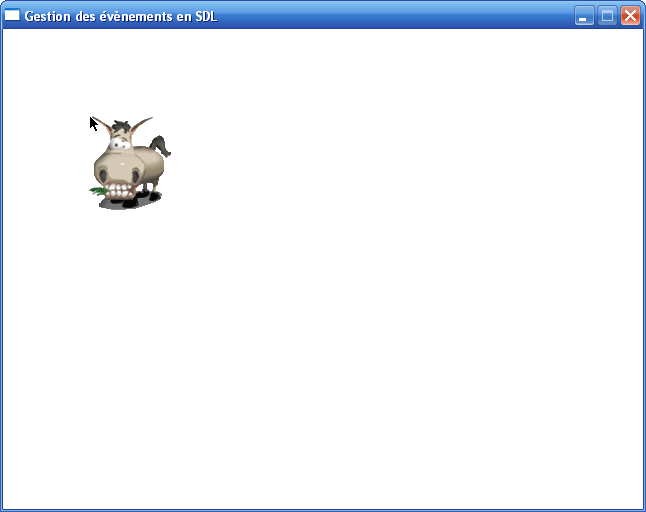
\includegraphics[width=0.6\textwidth]{Chapter_III-4_Window-Zozor-moved-mouse}
\end{figure}

إليك تمريناً سهلاً جداً : لحد الآن، نقوم بتحريك
\textenglish{Zozor}
مهما كان زر الفأرة الذي قمنا بضغطه. حاول ألا تحرّكه إلا إذا كان الزر المضغوط هو الأيسر. إذا تم الضغط على الزر الأيمن، يتوقف البرنامج.

\subsection{معالجة تحرّكات الفأرة}

تحرّك الفأرة يقوم بإنتاج حدث من نوع
\InlineCode{SDL\_MOUSEMOTION}.\\
و تيقن أنه يتم إنتاج أحداث بالقدر الذي تتحركه به الفأرة بيكسلا ببيكسل في الشاشة ! لو نحرّك الفأرة 100 بيكسل (هذا ليس كثيرا)، سيكون إذا هناك 100 حدث مـُنتج.

\begin{question}
لكن ألا تقوم هذه العملية بإنتاج الكثير من الأحداث بالنسبة للحاسوب ؟
\end{question}

لا بالتأكيد، تيقّن أنه يستقبل أكثر من ذلك بكثير !

حسناً، هل ما نقوم باسترجاعه مهم هنا ؟\\
إحداثيات الفأرة، بالطبع ! سنجدها في
\InlineCode{event.motion.x}
و
\InlineCode{event.motion.y}.

\begin{warning}
احذر : لن نعمل بنفس المركّبين اللذين استعملناهما من أجل النقر بالفأرة قبل قليل (سابقاً، كانت
\InlineCode{event.button.x}).
المركّبات المُستعملة تكون مختلفة في الـ\textenglish{SDL}
بحسب الحدث.
\end{warning}

سنقوم بتحريك
\textenglish{Zozor}
إلى نفس إحداثيات الفأرة، هنا أيضا. سترى أن العملية فعالة و بسيطة في نفس الوقت !

\begin{Csource}
while (cont)
{
	SDL_WaitEvent(&event);
	switch(event.type)
	{
		case SDL_QUIT:
		cont = 0;
		break;
		case SDL_MOUSEMOTION:
		zozorPosition.x = event.motion.x;
		zozorPosition.y = event.motion.y;
		break;
	}
	SDL_FillRect(screen, NULL, SDL_MapRGB(screen->format, 255, 255, 255));
	SDL_BlitSurface(zozor, NULL, screen, &zozorPosition); 
	SDL_Flip(screen);
}
\end{Csource}

حرّك
\textenglish{Zozor}
في الشاشة، ما رأيك ؟\\
سيتبع طبيعياً الفأرة أينما تتحرّك. هذا أمر جميل، سريع، و مرن (بفضل الـ\textenglish{double buffering}).

\subsection{دوال أخرى من أجل التعامل مع الفأرة}

سنرى دالتين سهلتي الاستعمال لهما علاقة بالفأرة. هاتان الدالتان ستكونان مفيدتين قريباً.

\subsubsection{إخفاء مؤشّر الفأرة}

يمكننا إخفاء مؤشر الفأرة بسهولة تامة، يكفي أن نستدعي الدالة
\InlineCode{SDL\_ShowCursor}
و نُعطيها عَلَماً~:

\begin{itemize}
	\item \InlineCode{SDL\_DISABLE} :
	إخفاء مؤشّر الفأرة.
	\item \InlineCode{SDL\_ENABLE} :
	إظهار مؤشر الفأرة.
\end{itemize}
مثلا :

\begin{Csource}
SDL_ShowCursor(SDL_DISABLE);
\end{Csource}

مؤشّر الفأرة سيبقى مختفياً طالما هو داخل النافذة.\\
أنصحك بأن تقوم بإخفائه قبل الحلقة الرئيسية في البرنامج لأنه لا داعي لإخفائه في كلّ دورة للحلقة، مرة واحدة كافية.

\subsubsection{وضع الفأرة في موضع محدد}

يمكننا تحريك مؤشر الفأرة يدويا إلى الإحداثيات التي نريدها في النافذة.\\
نستعمل من أجل هذا
\InlineCode{SDL\_WarpMouse}
و التي تأخذ كمعاملين الإحداثيتان
\InlineCode{x}
و 
\InlineCode{y}
أين يجدر بالمؤشّر أن يتواجد.

مثلا، الشفرة المصدرية التالية تقوم بتحريك الفأرة إلى وسط النافذة :

\begin{Csource}
SDL_WarpMouse(screen->w / 2, screen->h / 2);
\end{Csource}

\begin{information}
حينما تستدعي
\InlineCode{SDL\_WarpMouse}،
يتم إنتاج حدث من نوع
\InlineCode{SDL\_MOUSEMOTION}.
نعم، فالفأرة تحرّكت ! حتى و إن لم يقم المستعمل بذلك، فقد كان هناك تحرّك رغم ذلك.
\end{information}

\section{أحداث النافذة}

النافذة نفسها يمكن لها إنتاج عدد من الأحداث :

\begin{itemize}
	\item حينما يتم تغيير مقاييسها.
	\item حينما يتم إنزالها إلى شريط المهام السُفلي و حينما يتم استعادتها.
	\item حينما تصبح مفعّلة (شاشة أولى) أو حينما تصبح غير مفعلة.
	\item حينما يكون مؤشر الفأرة داخل النافذة أو حينما يخرُج منها.
\end{itemize}

فلنبدأ بدراسة الحالة الأولى : الحدثُ الذي يُنتج حينما يتم تغيير مقاييس النافذة.

\subsection{تغيير مقاييس النافذة}

بشكل افتراضي، تكون مقاييس النافذة غير قابلة للتعديل من طرف المستخدم.\\
أذكّرك بأنه لتغيير ذلك، يجب إضافة العَلم
\InlineCode{SDL\_RESIZABLE}
إلى الدالة
\InlineCode{SDL\_SetVideoMode}~:

\begin{Csource}
screen = SDL_SetVideoMode(640, 480, 32, SDL_HWSURFACE | SDL_DOUBLEBUF | SDL_RESIZABLE);
\end{Csource}

ما إن تتم إضافة هذا العَلم، يمكنك تغيير مقاييس النافذة. حينما تقوم بذلك، يتم إنتاج  حدث من نوع
\InlineCode{SDL\_VIDEORESIZE}.

يمكنك استرجاع :

\begin{itemize}
	\item العَرض الجديد من
	\InlineCode{event.resize.w}.
	\item الارتفاع الجديد من
	\InlineCode{event.resize.h}.
\end{itemize}

يمكننا استعمال هذه المعلومات من أجل أن نعمل على أن يكون
\textenglish{Zozor}
متمركزاً دائما في وسط النافذة :

\begin{Csource}
case SDL_VIDEORESIZE:
zozorPosition.x = event.resize.w / 2 - zozor->w / 2;
zozorPosition.y = event.resize.h / 2 - zozor->h / 2;
break;
\end{Csource}

\subsection{مرأى النافذة (\textenglish{Window visibility})}

يتم إنتاج الحدث
\InlineCode{SDL\_ACTIVEEVENT}
حينما يتم تغيير مرأى النافذة.\\
قد يحصل هذا لأسباب كثيرة :

\begin{itemize}
	\item حينما يتم إنزال النافذة إلى شريط المهام السفلي أو استرجاعها.
	\item تواجد مؤشر الفأرة داخل النافذة أو خارجها.
	\item حينما يتم تفعيل النافذة أو إلغاء ذلك.
\end{itemize}

\begin{information}
في البرمجة نتكلم عن
\textit{التركيز}
(\textenglish{Focus}).
حينما نقول أن تطبيقاً يملك التركيز، فهذا يعني أنه يستعمل لوحة المفاتيح أو الفأرة. و أي ضغط على أزرار لوحة المفاتيح أو نقر بالفأرة يتم إرسالها إلى النافذة التي بها التركيز و ليس لأخرى.\\
نافذة واحدة لها الحق في أن يكون لها تركيز في لحظة معيّنة (لا يمكن أن تكون نافذتان كشاشة أولى في آن واحد~!)
\end{information}

نظراً لكثرة الأسباب التي يمكن لها أن تسبب وقوع حدث ما، يجب قطعاً معرفة قيمة المتغيرات التالية لمعرفة المزيد :

\begin{itemize}
	\item \InlineCode{event.active.gain} :
تشير ما إن كان الحدث ربحا (1) أو خسارة (0). مثلاً، إذا انتقلت النافذة إلى الخلفية، فهذه خسارة (0) و إذا تم ارجاعها كشاشة أولى فهذا ربح (1).
	\item \InlineCode{event.active.state} :
	هو مزج بين عدة أعلام للإشارة إلى نوع الحدث الذي تم إنتاجه. هذه قائمة الأعلام الممكنة :
	\begin{itemize}
		\item \InlineCode{SDL\_APPMOUSEFOCUS} :
		مؤشّر الفأرة كان بصدد الدخول أو الخروج من النافذة. 
		يجب رؤية قيمة
		\InlineCode{event.active.gain}
		لنعرف ما إن كان قد دخل (ربح = 1) أو خرج (ربح = 0).
		\item \InlineCode{SDL\_APPINPUTFOCUS} :
		قامت النافذة باستقبال تركيز لوحة المفاتيح أو فقده. أي أنها انتقلت للخلفية أو رجعت كشاشة أولى.
		
		مرة أخرى، يجب رؤية قيمة 
		\InlineCode{event.active.gain}
		لنعرف ما إن تم وضع النافذة في الخلفية (ربح = 0) أو في الشاشة الأولى (ربح = 1).
		\item \InlineCode{SDL\_APPACTIVE} :
		تمت عملية
		\textit{أيقنة}
		النافذة، أي أنه تم إنزالُها إلى شريط المهام السفلي (ربح = 0) أو إرجاعها إلى مكانها الأصلي (ربح = 1).
	\end{itemize}
\end{itemize}

أمازلت تتابعني ؟ يجب مقارنة قيم المركّبات
\InlineCode{gain}
و
\InlineCode{state}
لمعرفة ما حصل بالفعل.

\subsubsection{اختبار قيمة الأعلام المدمجة}

\InlineCode{event.active.state}
هي عبارة عن دمج للأعلام. هذا يعني أنه في حدث، يمكن أن يحصل أمران (مثلاً، لو ننزل النافذة إلى شريط المهام، سنفقد تركيز لوحة المفاتيح و الفأرة أيضاً).\\
لهذا، يجب القيام باختبار أكثر تعقيدا من هذا :

\begin{Csource}
if (event.active.state == SDL_APPACTIVE)
\end{Csource}

\begin{question}
لماذا الأمر معقد ؟
\end{question}

لأنه عبارة عن مزج لبيتات 
(\textenglish{bits}).
لن أقوم بطرح درس حول العمليات المنطقية 
\textenglish{bit}
بـ\textenglish{bit}
الآن، لأنّ هذا سيكون كثيرا لهذا الدرس و ليس عليك معرفة الكثير عنها.\\
سأقدم لك شفرة قابلة للتطبيق و التي يجب عليك استعمالها إذا وُجد عَلمً في متغير دون الدخول في التفاصيل. 

لتجريب ما إن تم أي تغيير في التركيز الخاص بالفأرة مثلاً، يجدر بنا كتابة :  

\begin{Csource}
if ((event.active.state & SDL_APPMOUSEFOCUS) == SDL_APPMOUSEFOCUS)
\end{Csource}

لا توجد أخطاء. اِحذر، الأمر دقيق : يجب استعمال إشارة
\InlineCode{\&}
واحدة و اثنتين من
\InlineCode{=}،
و يجب استعمال الأقواس كما فعلت.

الشفرة تعمل بنفس الطريقة بالنسبة للأحداث الأخرى، مثلا :  

\begin{Csource}
if ((event.active.state & SDL_APPACTIVE) == SDL_APPACTIVE)
\end{Csource}

\subsubsection{اختبار الحالة و الربح في آن واحد}

عملياً، ستحتاج مؤكّدا إلى  اختبار الحالة و الربح في آن واحد. هكّذا يمكنك معرفة ما قد حصل بالفعل.

لنفترض أننا نبرمج لعبة تجعل الحاسوب يقوم بالكثير من الحسابات، تريد أن يتوقف البرنامج مؤقّتا تلقائيا عندما يتم إنزال النافذة إلى شريط المهام، ثم عند إعادتها إلى وضعها الأصلي، يُكمل البرنامج عمله تلقائياً. هذا سيجنبنا الحالة التي يستمر فيها البرنامج بالعمل حتى في غياب اللاعب، و سيجنبنا أيضاً جعل المعالج يقوم بالكثير من الحسابات التي لا فائدة منها.

الشفرة التالية تسمح للبرنامج بالتوقف قليلاً و ذلك بتفعيل المتغير المنطقي 
\InlineCode{pause}
(إعطائه القيمة 1). تقوم الشفرة بإكمال عمل البرنامج بتعطيل المتغير المنطقي (إعطائه القيمة 0).

\begin{Csource}
if ((event.active.state & SDL_APPACTIVE) == SDL_APPACTIVE)
{
	if (event.active.gain == 0) // If the window is minimized
		pause = 1;
	else if (event.active.gain == 1) // If the window is restored
		pause = 0;
}
\end{Csource}

\begin{information}
هذه الشفرة ليست كاملة بطبيعة الحال. عليك اختبار قيمة المتغير
\InlineCode{pause}
لمعرفة ما إن كان واجباً القيام بالحسابات في برنامجك أو لا.
\end{information}

سأترك لك القيام باختبارات من أجل الحالات الأخرى (مثلا، التأكد ما إن كان مؤشر الفأرة داخل أو خارج النافذة) يمكنك التدرّب و ذلك بتحريك
\textenglish{Zozor}
إلى اليمين إذا دخل مؤشّر الفأرة إلى النافذة و تحريكه إلى اليسار إذا خرج المؤّشر منها.

\section*{ملخّص}

\begin{itemize}
	\item الأحداث هي عبارة عن إشارات ترسلها إلينا الـ\textenglish{SDL}
	من أجل إطلاعنا على فعل قام به المستعمل~: الضغط على زر، تحريك أو النقر بالفأرة، غلق النافذة، إلخ.
	\item يتم استرجاع الأحداث في متغير من نوع
	\InlineCode{SDL\_Event}
	بواسطة الدالة
	\InlineCode{SDL\_WaitEvent}
	(دالة معطِّلة لكن يسهلُ التحكم بها) أو الدالة 
	\InlineCode{SDL\_PollEvent}
	(دالة غير معطِّلة لكن يصعب التحكم بها).
	\item يجب تحليل المركّب
	\InlineCode{event.type}
	من أجل معرفة نوع الحدث الذي تم إنتاجه. نقوم بذلك غالبا داخل 
	\InlineCode{switch}.
	\item ما إن يتم تحديد نوع الحدث، نحتاج غالبا إلى تحليل الحدث بالتفصيل. مثلا، عند الضغط على زر في لوحة المفاتيح
	(\InlineCode{SDL\_KEYDOWN})،
	يجب تحليل المركّب
	\InlineCode{event.key.keysym.sym}
	لمعرفة الزر الذي تم الضغط عليه بالضبط.
	\item تقنية الـ\textenglish{double buffering}
	هي تقنية تسمح بتحميل الصورة التالية في الشاشة الخلفية و إظهارها فقط حينما تكون جاهزة. هذا يسمح بتجنب تقطّع الصورة في الشاشة.
\end{itemize}
